% Тут еще нифига не готово :( %

% По умолчанию используется шрифт 14 размера. Если нужен 12-й шрифт, уберите опцию [14pt]
\documentclass[14pt]{matmex-diploma}
%\documentclass[14pt]{matmex-diploma-custom}

\usepackage{listings}
\usepackage{placeins}
\usepackage{color}
\usepackage{cite}

\definecolor{bluekeywords}{rgb}{0.13,0.13,1}
\definecolor{greencomments}{rgb}{0,0.5,0}
\definecolor{redstrings}{rgb}{0.9,0,0}

\lstdefinelanguage{FSharp}%
{morekeywords={let, new, match, with, rec, open, module, namespace, type, of, member, % 
and, for, while, true, false, in, do, begin, end, fun, function, return, yield, try, %
mutable, if, then, else, cloud, async, static, use, abstract, interface, inherit, finally },
  otherkeywords={ let!, return!, do!, yield!, use!, var, from, select, where, order, by },
  keywordstyle=\color{bluekeywords},
  sensitive=true,
  basicstyle=\ttfamily,
	breaklines=true,
  xleftmargin=\parindent,
  aboveskip=\bigskipamount,
	tabsize=4,
  morecomment=[l][\color{greencomments}]{///},
  morecomment=[l][\color{greencomments}]{//},
  morecomment=[s][\color{greencomments}]{{(*}{*)}},
  morestring=[b]",
  showstringspaces=false,
  literate={`}{\`}1,
  stringstyle=\color{redstrings},
}

\begin{document}
% Год, город, название университета и факультета предопределены,
% но можно и поменять.
% Если англоязычная титульная страница не нужна, то ее можно просто удалить.
\filltitle{ru}{
    chair              = {Кафедра системного программирования},
    title              = {Реализация библиотеки парсер-комбинаторов на основе алгоритма для платформы .NET},
    % Здесь указывается тип работы. Возможные значения:
    %   coursework - Курсовая работа
    %   diploma - Диплом специалиста
    %   master - Диплом магистра
    %   bachelor - Диплом бакалавра
    type               = {coursework},
    position           = {студента},
    group              = 371,
    author             = {Мелентьев Кирилл Игоревич},
    supervisorPosition = {ст. преп., магистр информационных технологий},
% * <melentyev.k@gmail.com> 10:52:49 23 May 2016 UTC+0300:
% Как правильно записать?
    supervisor         = {Григорьев С.В.},
    %reviewerPosition   = {ст. преп.},
    %reviewer           = {Привалов А.\,И.},
    %chairHeadPosition  = {д.\,ф.-м.\,н., профессор},
    %chairHead          = {Хунта К.\,Х.},
%   university         = {Санкт-Петербургский Государственный Университет},
%   faculty            = {Математико-механический факультет},
%   city               = {Санкт-Петербург},
%   year               = {2013}
}
%\filltitle{en}{
%    chair              = {The Meaning of Life \\ Uselessness of Everything},
%    title              = {Empty subset as closed set},
%    author             = {Edelweis Mashkin},
%    supervisorPosition = {professor},
    %supervisor         = {Amvrosy Vibegallo},
    %reviewerPosition   = {assistant},
    %reviewer           = {Alexander Privalov},
    %chairHeadPosition  = {professor},
    %chairHead          = {Christobal Junta},
%}
\maketitle
\tableofcontents
% У введения нет номера главы
\section*{Введение}
Традиционно, для создания синтаксических анализаторов используются генераторы 
синтаксических анализаторов, при этом используется особый язык спецификации 
грамматики, а семантические действия, как правило, 
описываются на другом языке программирования.
Известным примером является Yacc \cite{johnson1975yacc} --- генератор синтаксических анализаторов на языке C 
(существует множество клонов yacc, генерирующих синтакисческие анализаторы на других языках). \ 
Другой подход --- парсер-комбинаторы --- подход, при котором, парсер строится динамически, 
из простейших парсеров с использованием функций комбинирующих их. Парсер-комбинаторы позволяют 
реализовать синтаксический анализатор и семантические действия на одном языке, 
на котором пишется дальнейшая обработка данных. 
Более того, этот подход обладает другими преимуществами: 
  естественность и понятность описания анализаторов, а также простота отладки,
  обеспечиваемая свойством модульности. 

Однако многие библиотеки парсер-комбинаторов
  (например классическая библиотека парсер-комбинаторов Parsec \cite{LeijenMeijer:parsec} для Haskell, 
  или библиотека FParsec \cite{fparsec} для F\#), 
  наследуя свойство нисходящих синтаксических анализаторов,  
  не поддерживают леворекурсивные правила грамматик 
  или испытывают проблемы с производительностью
  при использовании неоднозначных грамматик. 
  Многие стандартные грамматики содержат леворекурсивные правила, например грамматика арифметических выражений, 
  выражений с постфиксными операциями --- вызовами функций,
  обращениями к элементам массива по индексу, 
обращения к полям структуры/объекта. В общем случае, если парсер-комбинаторы не поддерживают леворекурсивные правила, 
то придется модифицировать грамматику, удалив леворекурсивные правила, 
а так же изменить семантические действия. Необходимость этих действий может усложнить разработку, увеличить время разработки. В данной работе мы рассмотрим реализацию одного из решений этой проблемы под платформу .NET.


\section{Обзор существующих решений}

В данной курсовой работе были рассмотрены возможности и свойства, следующих популярных библиотек парсер-комбинаторов: 
FParsec (для F\#), Attoparsec \cite{attoparsec} (для Haskell), gll-combinators \cite{gllcombinators} (для Scala). Каждая из библиотек обладает различными особенностями, среди которых были выделены следующие характерные возможности: 
построение синтаксического анализаторы на основе грамматики, содержащей леворекурсивные правила; 
  поддержка работы с абстрактным типом входных данных 
  (многие библиотеки парсер комбинаторов позволяют работать только с потоком символов); 
  Возможность создания инкрементальных синтаксических анализаторов.

\subsection{Леворекурсивные правила}

Различные библиотеки парсер-комбинаторов предоставляют свои решения проблемы с леворекурсивными правилами, например FParsec имеет специальный интерфейс OperatorPrecedenceParser для создания парсеров арифметических выражений с инфиксными, префиксными и постфиксными операторами. Но непосредственно работать с леворекурсивными правилами (среди рассмотренных решений) умеет только библиотека gll-combinators (Scala), которая и была взята за основу нашего решения.

\subsection{Абстрактный тип входа}

Возможность работы с абстрактным типом входных данных расширяет набор возможных способов использования библиотеки, 
например символы входного потока могут быть дополнены какой-либо важной для анализатора мета-информацией.
Также, в каких-то случаях, может быть удобно работать с потоком лексем поступающих от лексического анализатора --- 
во-первых синтаксический анализатор упрощается благодаря тому,
что лексический анализатор сам обрабатывает и фильтрует такие конструкции, 
как пробелы и комментарии в исходном коде; во-вторых, возможно повышение 
производительности, так как лексический анализатор обычно работает 
быстро благодаря более простой конструкции, и длина входного потока, 
поступающего синтаксическому анализаторы в разы меньше, чем длина текста в символах.

\subsection{Инкрементальный анализ}
Библиотека Attoparsec позволяет создавать инкрементальные лексические 
анализаторы. Работают анализаторы Attoparsec так: когда анализатор встречает конец входного потока (при этом ожидая 
какого-либо символа) он остановливается и возвращает новый парсер, 
который можно применить к новому входному потоку так, будто бы это 
продолжение предыдущего. Например, пусть мы сконктруировали парсер X 
для арифметических выражений:
\begin{lstlisting}
E ::= E ('+' | '-') T | T
T ::= T ('*' | '/') F | F
F ::= num | '(' E ')' 
\end{lstlisting}
Применив X к строке "2+(", мы получим парсер Y. 
Применив парсер Y к строке "3-4)", мы получим итоговый результат для строки "2+(3-4)". 

Такой подход может быть удобен в случаях, когда входной поток не доступен 
весь в один момент, а поступает частями, например при получении данных по сети --- 
пакеты могут быть обработаны последовательно, нет необходимости собирать весь 
входной поток в один буффер.
Другим примером использования может быть анализ исходного кода в IDE 
(для подсветки синтаксических конструкций): например можно сохранять 
промежуточные результаты анализа для каждой n-ой позиции, и когда 
пользователь редактирует код в одном месте, не нужно заново анализировать 
весь файл --- можно продолжить парсинг от ближайшего сохраненного 
анализатора (придется откинуть следующие за ним).


\subsection{gll-combinators}
Рассмотрим, каким образом библиотека gll-combinators справляется с произвольными КС-грамматиками.
В основе реализации этой библиотеки лежит алгоритм GLL, 
  разработанный в 2009 учеными Elizabeth Scott и Andrian Johnstone \cite{gllsj}. 
GLL --- это разновидность нисходящего рекурсивного спуска, 
  благодаря чему он может быть адаптирован для использования комбинаторами парсеров. 
Алгоритм имеет асимптотику  $O(n^3)$ в худшем случае, в отличие от обыкновенного 
  рекурсивного спуска с возвратом, который в худшем случае имеет экспоненциальную сложность.
  
Daniel Spiewak, автор библиотеки gll-combinators, адаптировал  GLL 
  под подход парсер-комбинаторов и разработал реализацию на Scala, на которой и основывается наша работа. 
  


\section{Постановка задачи}
Целью данной курсовой работы является разработка библиотеки парсер-комбинаторов,
поддерживающих произвольные контекстно-свободные грамматики, для платформы .NET.
Для достижения данной цели поставлены следующие задачи.
\begin{itemize}
    \item Разработать библиотеку парсер-комбинаторов со следующими свойствами и возможностями:
    \begin{itemize}
        \item платформа реализации .NET;
        \item возможность создания синтаксических анализаторов на основе произвольных контекстно-свободных грамматик;
        \item поддержка работы с абстрактным типом входных данных;
        \item возможность создания инкрементального синтаксических анализаторов.
    \end{itemize}
    \item Провести сравнение производительности с существующими решениями.
\end{itemize}


\section{Реализация}
В ходе курсовой работы была данная библиотека была реализована (далее FsGll). Приводятся некоторые детали ее реализации и использования.

\subsection{Детали реализации}
Реализация базовой части библиотеки повторяет реализацию описанную Daniel Spiewak,
за исключением некоторых технических моментов, связанных с использованием языка F\#, 
а также с использованием произвольного типа входа. 

Реализация инкрементальной версии потребовала небольших модификаций алгоритма. 
Во-первых, были заменены структуры данных, основанные на хэш-таблицах, на структуры данных,
основанные на деревьях поиска
(множества и ассоциативные массивы). Так же все функции, модифицировавшие состояние процесса синтаксического анализа, 
стали возвращать новый объект состояния. Суть модификации непосредственно алгоритма в следующем: 
когда анализатор возвращает ошибку конца входного потока, то
вместо того, чтобы вызвать для этой ошибки функцию обрабатывающую результат, мы добавляем 
этот анализатор и функцию обработки в список (хранящийся в объекте, 
инкапсулирующем состояние процесса анализа) для "перезапуска" при запуске на следующей части входного потока. 
В конце процесса (когда все пути анализа пройдены) проверяется, не пуст ли данный список 
"перезапуска", и если он не пуст, то в список результатов 
добавляется PartialParser, сохранивший этот список.



\subsection{Интерфейс библиотеки}
Интерфейс библиотеки FsGll предоставляет типы и функции в нескольких пространствах имен:
\begin{itemize}
    \item {\tt FsGll.Parsers} --- базовая реализация 
    (не предоставляющая возможности для создания инкрементальных анализаторов) на основе изменяемых структур данных;
    \item {\tt FsGll.Parsers.Incremental} --- реализация парсер-комбинаторов для 
          инкрементального анализа на основе изменяемых структур;
    \item {\tt FsGll.Parsers.Incremental.Pure} --- реализация парсер-комбинаторов для 
          инкрементального анализа на основе неизменяемых структур.
\end{itemize}

Все эти пространства имен предоставляют тип {\tt Parser<'a,'r>}, экземплярами которого являются парсеры.
\begin{itemize}
    \item {\tt 'a} --- тип возвращаемого парсером значения.
    \item {\tt 'r} --- тип элементов входного потока.
\end{itemize}

FsGll.Parsers предоставляет тип {\tt Result<'a,'r>} для описания результата синтаксического анализа:
\begin{lstlisting}[language=FSharp]
type Result<'a,'r> = Success of 'a
    	           | Failure of string * Stream<'r>
\end{lstlisting}

Далее приведены некоторые комбинаторы и функции, используемые в примере.
\begin{itemize}
    \item {\tt runParser<'a, 'r>: Stream<'r> -> [Result<'a,'r>] } --- Функция  предназначена для запуска анализатора на входном потоке. Она возвращает список всех успешных результатов анализа (поскольку на неоднозначной грамматике их может быть много), либо список всех ошибок.
    \item {\tt satisfy: ('a -> bool) -> Parser<'a,'r>} --- принимает или отвергает элемент входного потока 
    \item {\tt (<|>) : Parser<'a,'r> -> Parser<'a,'r> -> Parser<'a,'r> } --- альтернатива.
    \item {\tt (>}{\tt >=) : Parser<'a,'r> -> ('r -> Parser) -> Parser<'a,'r2>} --- связывание.
    \item {\tt createParserForwardedToRef} --- аналог соответствующей функции из пакета FParsec
        \cite{fparsec:createpforwtoref}.
\end{itemize}
(полный список на странице документации \cite{fsglldoc})\\

Пространства имен {\tt FsGll.Parsers.Incremental} и \sloppy {\tt FsGll.Parsers.Incremental.Pure} 
расширяют тип {\tt Result}, добавляя конструктор {\tt Partial} 
(соответственно функции {\tt runParser} в этих пространствах имен также могут 
в списке результатов вернуть {\tt Partial}):

\begin{lstlisting}[language=FSharp]
type Result<'a,'r> = Success of 'a
    	           | Failure of string * Stream<'r>
                   | Partial of Parser<'a,'r>
\end{lstlisting}

Далее приведен пример использования комбинаторов из \sloppy {\tt FsGll.Parsers.Incremental.Pure} 
(интерфейсы парсер-комбинаторов из других пространств имен аналогичны за исключением
отсутствия {\tt Partial} результата в {\tt FsGll.Parsers}) для описания синтаксического анализатора языка арифметических выражений с односимвольными операндами и операциями (+, -, *, /) по следующей грамматике:
\begin{lstlisting}
E ::= E ('+' | '-') T | T
T ::= T ('*' | '/') F | F
F ::= num | '(' E ')' 
\end{lstlisting}

Исходный код примера:
\begin{lstlisting}[language=FSharp]
// utilities
let isPartial = function Partial(_) -> true 
                       | _          -> false
let getPartial = List.tryFind isPartial
let parse p s = runParser<_,_> p (stringStream s)

// construct parser
let e, er = createParserForwardedToRef<_>()
let t, tr = createParserForwardedToRef<_>()
let chr c = satisfy ((=)c) 
let op = chr '+' <|> chr '-' 
     <|> chr '*' <|> chr '/'
let num = satisfy (Char.IsDigit) |>> Int32.Parse
let f = num <|> (chr '(' >>. e .>> chr')')

let sem l x r = 
    match x with 
    | '+' -> l + r 
    | '-' -> l - r
    | '*' -> l + r 
    | '/' -> l - r
    
er := pipe3 e op t sem <|> t
tr := pipe3 t op f sem <|> f

// run
let f = parse e "1+2*" |> getPartial 
let g = parse f "(3" |> getPartial
let h1 = parse f "3+4"
let h2 = parse g "+4)"
\end{lstlisting}

Анализатор применяется к строке {\tt "1+2*"}, которая не принадлежит языку 
  (но может быть дополнена до корректной), после чего из списка результатов 
  извлекается новый анализатор f, который применяется к продолжению строки 
  ({\tt "(3"}) для получения следующего "промежуточного" анализатора g. Анализатор f также
  применяется к {\tt "3+4"}, после чего в списке результатов h1 содержится корректный
  результат 11. Анализатор g применяется к {\tt "+4)" }, и возвращает корректный результат 15.






\section{Замеры производительности}

Тестирование проводилось на компьютере со следующими характеристиками:
\begin{itemize}
    \item CPU --- Intel Core i5-5300U;
    \item RAM --- 12 Гб.
\end{itemize}
Каждый тест запускался отдельным процессом, каждый раз предварительно «разогревая» runtime 
систему коротким тестом.\\

Первое сравнение проводилось между FsGll и gll-combinators на следующей 
сильно неоднозначной грамматике, содержащей леворекурсивные правила: 
\begin{lstlisting}
S ::=  S  S  S 
    |  S  S 
    | '0'
\end{lstlisting}

График производительности представлен на изображении (рис.~\ref{nnn_scala_fsgll}).
Результаты сравнения демонстрируют, что производительность обоих решений на данной грамматике сопоставима. 
% * <melentyev.k@gmail.com> 14:39:12 25 May 2016 UTC+0300:
% Я не понял что произошло.. Надо удалить строчку?

\begin{figure}[!h]
  \label{nnn_scala_fsgll}
  \centering
  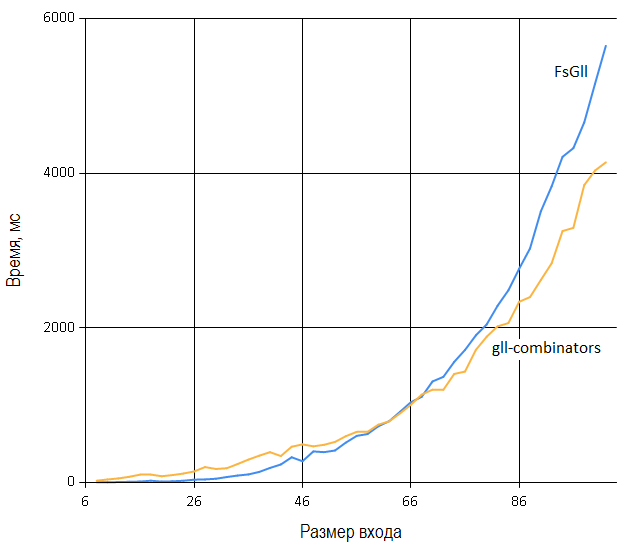
\includegraphics[width=15cm]{pics/graph1.png}
  \caption{Сравнение производительности FsGll и gll-combinators на сильно неоднозначной грамматике}
\end{figure}
\FloatBarrier




Следующий тест сравнивает производительность  FsGll и FParsec на грамматике арифметических выражений:
\begin{lstlisting}
E ::= E (‘+’ | ’-‘) T | T
T ::= T (‘*’ | ‘/’) F | F
F ::= ident | value | '(' E ')'
Stmt ::= ident '=' Expr ';'
P ::= Stmt* E
\end{lstlisting}

График производительности представлен на изображении (рис.~\ref{ec_fparsec_fsgll_1}). 
Здесь "Размер входа" --- это количество операндов в выражении.

\begin{figure}[!h]
  \label{ec_fparsec_fsgll_1}
  \centering
  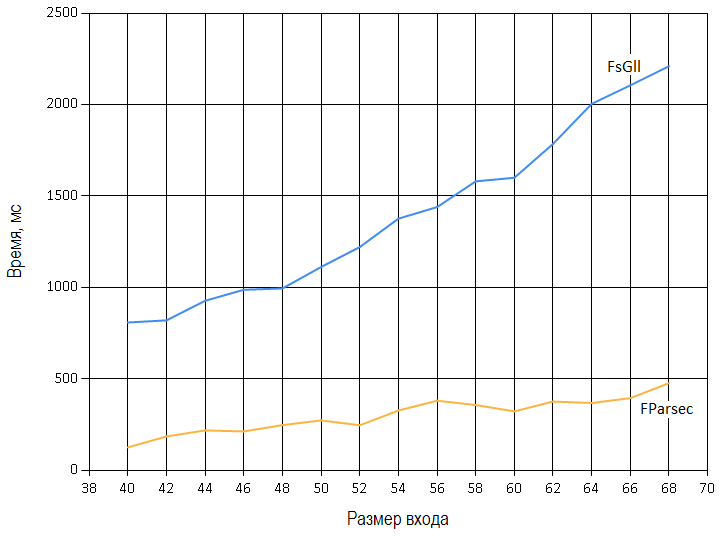
\includegraphics[width=15cm]{pics/graph2.png}
  \caption{Сравнение производительности FParsec и FsGll на грамматике арифметических выражений}
\end{figure}
\FloatBarrier

Результаты сравнения демонстрируют, что по производительности на данном примере FParsec значительно превосходит FsGll. FParsec --- промышленная библиотека, довольно хорошо работает на стандартных грамматиках. Предстоит дальнейшая работа по опимизации FsGll, для достижения сопоставимых результатов.
\\
Последний тест сравнивает производительность реализаций, предназначенных для создания 
инкрементальных парсеров. Грамматика вновь:
\begin{lstlisting}
S ::=  S  S  S 
    |  S  S 
    | '0'
\end{lstlisting}
Символы подаются на вход по одному. 
График производительности представлен на изображении (рис.~\ref{nnn_fsgll_incr}). \\

	
\begin{figure}[!h]
  \label{nnn_fsgll_incr}
  \centering
  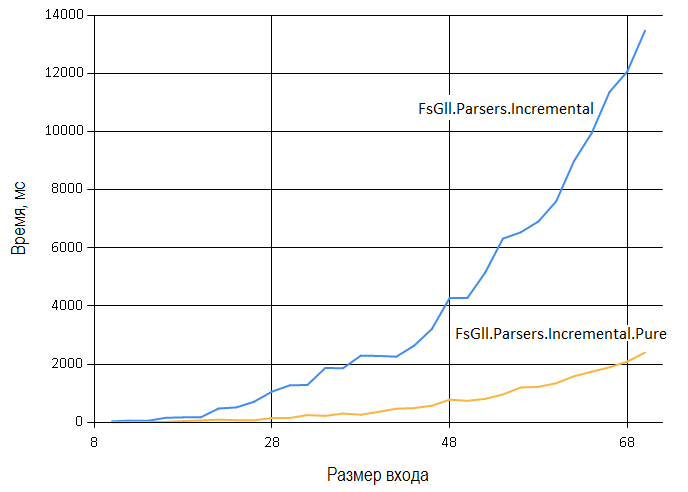
\includegraphics[width=15cm]{pics/graph3.png}
  \caption{Сравнение производительности FsGll.Parsers.Incremental и FsGll.Parsers.Incremental.Pure на сильно неоднозначной}
\end{figure}
\FloatBarrier

Производительность решения реализованного на основе неизменяемых структур данных ожидаемо ниже, 
в текущей реализации в 6 раз.



% У заключения нет номера главы
\section*{Заключение}
В рамках данной курсовой работы была реализована библиотека парсер-комбинаторов 
для платформы .NET, FsGll, обладающая следующими возможностями:
\begin{itemize}
    \item возможность создания синтаксических анализаторов на основе произвольных КС грамматик
    \item поддержка работы с абстрактным типом входных данных 
    \item возможность создания инкрементального синтаксических анализаторов.
\end{itemize}

Библиотека сочетает в себе возможности различных существующих библиотек, 
благодаря чему является довольно универсальным решением. 

Также было проведено сравнение производительности с другими известными библиотеками парсер-комбинаторов.
Производительность данного решения сравнима со своим прообразом (gll-combinators), 
но проигрывает другим библиотекам, при использовании сходных грамматик. В качестве дальнейшего развития возможна работа по оптимизации производительности библиотеки. 

По результатам данной работы был представлен доклад на конференции 
"Современные технологии в теории и практике программирования" в СПбПУ.

\begin{itemize}
    \item Исходный код библиотеки доступен по ссылке (пользователь melentyev): https://github.com/YaccConstructor/FsGll
    \item Документация: http://yaccconstructor.github.io/FsGll/
    \item NuGet пакет: https://www.nuget.org/packages/FsGll/
\end{itemize}
%\cite{fsgllgit} \cite{fsglldoc} \cite{fsgllpack}


\setmonofont[Mapping=tex-text]{CMU Typewriter Text}
\bibliographystyle{ugost2008ls}
\bibliography{diploma.bib}
\end{document}
